\documentclass[border=10pt]{standalone}
\usepackage{tikz}
\usetikzlibrary{arrows.meta,positioning,shapes.geometric}

\begin{document}
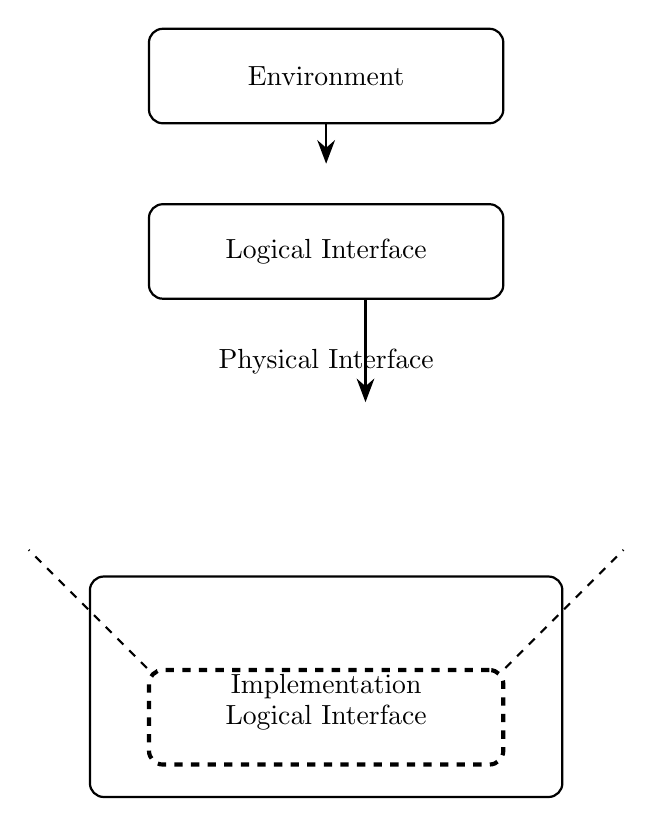
\begin{tikzpicture}[
    node distance=1.5cm and 2cm,
    box/.style={rectangle, draw=black, thick, rounded corners=5pt, 
                minimum width=4.5cm, minimum height=1.2cm, align=center},
    dashed box/.style={box, dashed, line width=1.5pt},
    arrow/.style={-{Stealth[length=3mm]}, thick}
]

% Top box - Environment
\node[box] (env) at (0,0) {Environment};

% Arrow from Environment to Logical Interface
\draw[arrow] (env.south) -- ++(0,-0.5);

% Middle box - Logical Interface
\node[box, below=1cm of env] (logical) {Logical Interface};

% Physical Interface text (not boxed)
\node[below=0.5cm of logical] (physical) {Physical Interface};

% Arrow from Logical Interface to Implementation
\draw[arrow] ([xshift=0.5cm]logical.south) -- ++(0,-1.3);

% Bottom box - Implementation
\node[box, below=3.5cm of logical, minimum width=6cm, minimum height=2.8cm] (impl) {Implementation};

% Dashed box for Logical Interface inside Implementation
\node[dashed box, above=0.4cm of impl.south] (logical2) {Logical Interface};

% Dashed arrows from both sides connecting to top Logical Interface
\draw[thick, dashed] (logical2.north west) -- ++(-1.5,1.5);
\draw[thick, dashed] (logical2.north east) -- ++(1.5,1.5);

\end{tikzpicture}
\end{document}
